\documentclass[12pt]{article}
\usepackage[a4paper]{geometry}
\usepackage[utf8]{inputenc}
\usepackage{fancyhdr}
\usepackage{lastpage}
\usepackage{graphicx, wrapfig, subcaption, setspace, booktabs}
\usepackage{graphicx}
\usepackage[T1]{fontenc}
\usepackage[font=small, labelfont=bf]{caption}
\usepackage[protrusion=true, expansion=true]{microtype}
\usepackage[english]{babel}
\usepackage{sectsty}
\usepackage{url, lipsum}
\usepackage[T1]{fontenc}
\usepackage{icomma}
\usepackage{siunitx}
\usepackage{ragged2e}
\usepackage{amsmath}
\usepackage{comment}
\usepackage{enumerate}
\usepackage{anysize}
\usepackage{graphicx}
\usepackage{amssymb}
\usepackage{apacite}
\bibliographystyle{apacite}
\newcommand{\HRule}[1]{\rule{\linewidth}{#1}}
\onehalfspacing
\setcounter{tocdepth}{5}
\setcounter{secnumdepth}{5}
\usepackage[utf8]{inputenc}
\usepackage{amssymb}
\usepackage{graphicx}
\usepackage{amsmath}
\onehalfspacing
\setcounter{tocdepth}{5}
\setcounter{secnumdepth}{5}

%-------------------------------------------------------------------------------
% HEADER & FOOTER
%-------------------------------------------------------------------------------


\begin{comment}
-Udledninger
$$
\begin{aligned}
\end{aligned}
$$

-Opgavetekst
\begin{figure}[H]
\includegraphics[width=0.5\textwidth]{"path"}
\end{figure} 


-Opgave billede med tekst
\begin{figure}[H]
\caption{"Billedtekst"}
\includegraphics[width=0.5\textwidth]{"path"}
\end{figure} 

-Værdier
$\\
$


\end{comment}
\begin{document}

\begin{titlepage}

\title{ \normalsize 
		%\begin{figure}
        \begin{center}
        
\includegraphics[height=6cm]{Logo.jpg}
        \end{center}
       % \end{figure}
        \LARGE \textsc{\textbf{Universidad De Sonora}} \\ \bigskip
		\Large División de Ciencias Exactas y Naturales \\
        Licenciatura en Física \\ \bigskip
        \bigskip
        Física Computacional I
		\\ [0.1cm]  
		\HRule{2pt} \\
		\Large \textbf{{Actividad 10}} \\
        \textit{\textbf{"Solución Numérica de Ecuaciones Diferenciales Parciales."}}
		\HRule{2pt} \\
		\normalsize \vspace*{0.001\baselineskip}}
        
\date{\bigskip \Large  \hspace*{\fill} Hermosillo, Sonora a abril 10 de 2021}

        
\author{
		\Large\textbf{Ismael Espinoza Arias} \\ \bigskip
        \\ \bigskip
       \Large Profesor Carlos Lizárraga Celaya}
       \end{titlepage}
       \maketitle
       
       
%-----------------------------------------------------------


\section*{Introducción y Antecedentes}
La mayoría de los problemas físicos y de ingeniería de importancia práctica están descritos por este tipo de ecuaciones diferenciales, y fundamentalmente por ecuaciones diferenciales de segundo orden. Por ello el tratamiento de las EDP que se desarrollará en lo sucesivo se concentrará sobre ecuaciones lineales de segundo orden. Las ecuaciones diferenciales de segundo orden en derivadas parciales pueden expresarse de forma general como: 

\begin{center}
    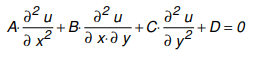
\includegraphics[height=2cm]{ED.png}\\
\end{center}

Para resolver esta ecuación hay que tener en cuenta la distribución inicial de temperaturas en el cuerpo y las condiciones de contorno. Se deduce también, la ecuación de la conducción del calor cuando el cuerpo genera internamente calor por algún procedimiento.

n matemáticas una ecuación en derivadas parciales (a veces abreviada como EDP) es aquella ecuación diferencial cuyas incógnitas son funciones de diversas variables independientes, con la peculiaridad de que en dicha ecuación figuran no solo las propias funciones sino también sus derivadas. Tienen que existir funciones de por lo menos dos variables independientes.1. O bien una ecuación que involucre una función matemática ${\displaystyle u}u$ de varias variables independientes x, y, z, …, y las derivadas parciales de u respecto de esas variables. Las ecuaciones en derivadas parciales se emplean en la formulación matemática de procesos de la física y otras ciencias que suelen estar distribuidos en el espacio y el tiempo. Problemas típicos son la propagación del sonido o del calor, la electrostática, la electrodinámica, la dinámica de fluidos, la elasticidad, la mecánica cuántica y muchos otros. Se las conoce también como ecuaciones diferenciales parciales. Participaron, al inicio, en su estudio los franceses d'Alembert, Fourier, matemáticos de la época napoleónica.


%-----------------------------------------------------------


\section*{Ecuación del calor}

Resolveremos por el método de diferencias finitas la Ecuación del Calor en una dimensión para la temperatura u(t,x), dada una condición inicial y 2 condiciones a la frontera. Por ejemplo una barra de cobre de longitud L=1 (térmicamente aislada en las paredes), y los extremos pueden estar térmicamente aislados, o estar a cierta temperatura fija, o estar libres para que el calor escape.

\begin{center}
    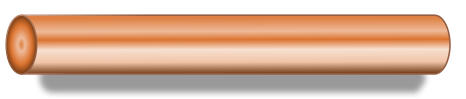
\includegraphics[height=2cm]{EC.png}
\end{center}

Por ejemplo la Ecuación del Calor para una barra de longitud 1, con temperatura fija de 0ºC en los extremos (en contacto con una barra de hielo), y habiendo una distribución de temperatura inicial dentro de la barra descrita por la función f(x). 

\begin{center}
    $U_{t}(x,t) = KU_{xx}(x,t)$\\
    $U(0,t) = U(1,t) = 0$\\
    $U(x,0) = f(x)$\\
\end{center}


%-----------------------------------------------------------


\subsection*{Importación de bibliotecas}
Empezamos importando nuestras bibliotecas, el primer paso para empezar con cualquier actividad.

\begin{center}
    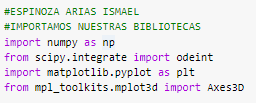
\includegraphics[height=4cm]{Bibliotecas.png}
\end{center}
 
 Donde podemos ver que las bibliotecas utilizadas, son numpy, scipy, matplotlib, toolkits, ect. Donde nos ayudaran a resolver nuestro siguiente problema.


%-----------------------------------------------------------


\subsection*{Realización de la actividad}
Ahora para la actividad, vamos a definir nuestros valores y resolver la ecuación del calor usando ecuaciones diferenciales parciales.


 

%--------------------------1---------------------------------


\subsection*{Ejercicio 1}

Para el caso $a)$ tenemos una barra metálica de longitud $L = 10$, y coeficiente de difusión  $k = 100$ . Condición inicial (Temperatura dentro de la barra): $u(x,0) = 0$. Condiciones a la frontera: $u(0,t) = 10, u(L,t) = 0$. Realice los cálculos hasta alcanzar el equilibrio térmico.

\begin{center}
    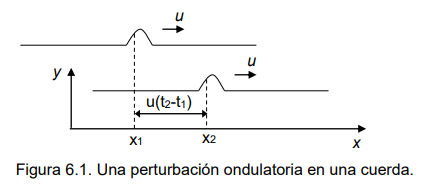
\includegraphics[height=8cm]{E1.png}
\end{center}

Relizando las operaciones correspondientes, llegamos a la gráfica siguiente:

\begin{center}
    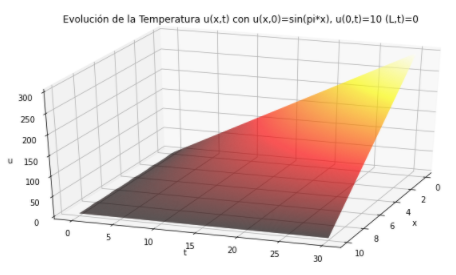
\includegraphics[height=8cm]{Grafica1.png}
\end{center}


Para el caso $b)$ tenemos un material de longitud $L=10$ con coeficiente de difusión térmica $\kappa=0.25$ Condición inicial u(x,0)=20. Condiciones a la frontera: u(0,t)=(20 + 10 sin(pi*t/12), u(L,t)=20. Realice los cálculos para t=(0,48) Pueden ajustar los parámetros para ver cómo cambia la temperatura dentro del cuerpo.

\begin{center}
    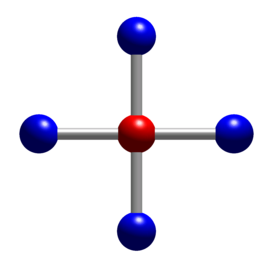
\includegraphics[height=8cm]{E2.png}
\end{center}

Relizando las operaciones correspondientes, llegamos a la gráfica siguiente:

\begin{center}
    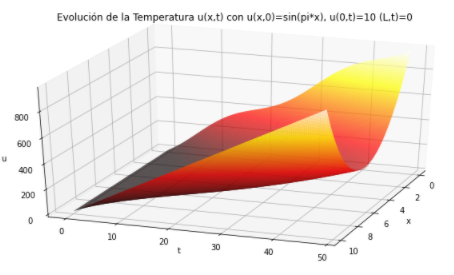
\includegraphics[height=8cm]{Grafica2.png}
\end{center}


Para el caso $c)$ Implementamos la diferencias finitas para esta ocasión.

\begin{center}
    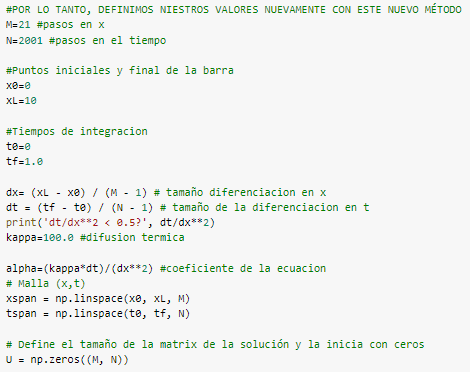
\includegraphics[height=10cm]{E3.png}
\end{center}

Relizando las operaciones correspondientes, llegamos a la gráfica siguiente:

\begin{center}
    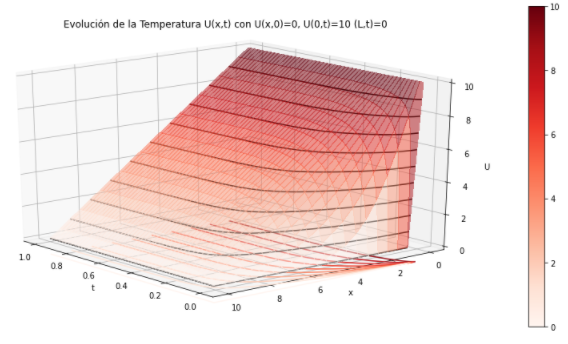
\includegraphics[height=8cm]{Grafica3.png}
\end{center}


Para el caso $d)$ Implementamos la diferencias finitas para esta ocasión.

\begin{center}
    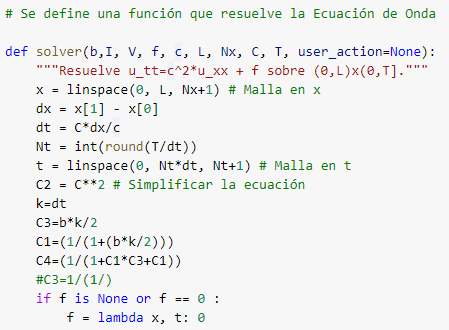
\includegraphics[height=10cm]{E4.png}
\end{center}

Relizando las operaciones correspondientes, llegamos a la gráfica siguiente:

\begin{center}
    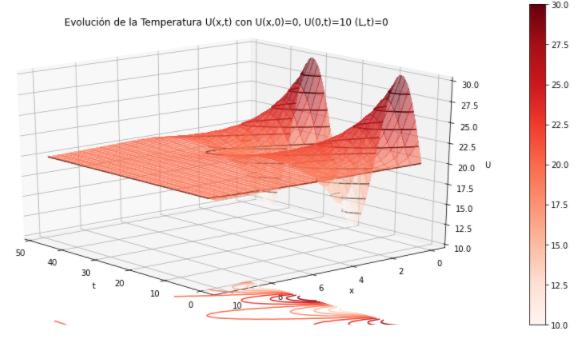
\includegraphics[height=8cm]{Grafica4.png}
\end{center}


%-----------------------------------------------------------


\subsection*{Ejercicio 2}

Variaciones de la Temperatura en el Suelo. La superficie de la Tierra recibe radiación solar durante el día. Esta Energía la transforma en calor, y cambia la temperatura dentro del suelo. Por la noche al no recibir radiación solar la emite a la atmósfera. 

Si suponemos que la temperatura del suelo varía con la profundidad, podemos suponer que tenemos un problema unidimensional, siendo el eje $x$ la dirección hacia dentro del suelo.

A cierta profundidad $x=L$, suponemos que la temperatura ya no cambia, es decir $\partial u/\partial x = 0$ (Condición de Neumann).

Supondremos que la variación de la temperatura en la superficie terrestre varía como 

\begin{equation*}
u(0,t) = u_0 + u_a \sin (\frac{2\pi t}{P})
\end{equation*}

donde $u_0$ es la inical temperatura promedio del suelo y $u_a$ es la temperatura del aire. La constante $P$ es el periodo de variación diaria de temperatura $P=24 h=86,400 s$.

En este caso la constante de difusión de calor es $\kappa = 1.0 \times 10^{-6}$. El tiempo será medido en segundos. 

Usando la Ecuación de Calor, determina numéricamente  la variación del perfil de temperatura dentro del suelo, por ejemplo para Hermosillo en estos días supongamos que $u_0=15^{o}C$, $u_a= 20^{o}C$. Realiza una simulación de al menos 48 horas. 

\begin{center}
    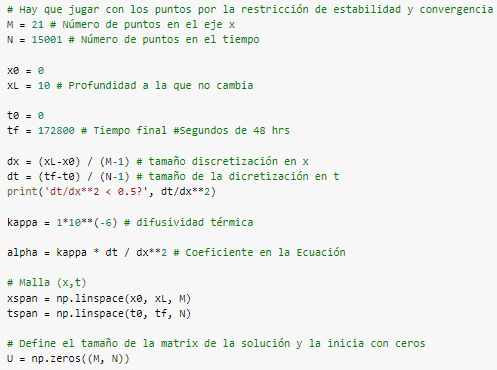
\includegraphics[height=8cm]{E5.png}
\end{center}

Relizando las operaciones correspondientes, llegamos a la gráfica siguiente:

\begin{center}
    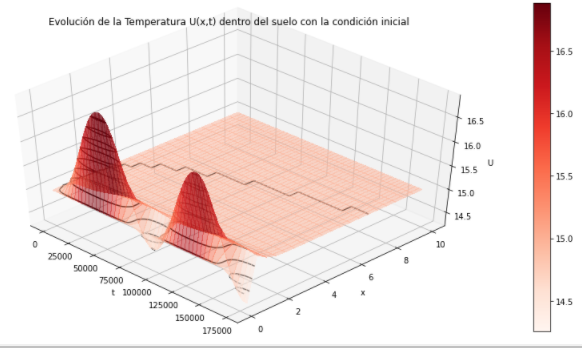
\includegraphics[height=8cm]{Grafica5.png}
\end{center}


%-----------------------------------------------------------
\newpage

\section*{Conclusiones, resultados y discusión}
En esta activiadad se reforzaron los conocimientos adquridos en las clases de teoría, impartidas por el docente en el transcruso de la semana. En esta ocasión resolvimos y aplicamos algunos ejemplos de la ecuación de calor, donde graficamos las soluciones viendo como es que estas se comportan. También vimos 2 métodos aplicamos para realizar este ejercicio y de una forma utilizando las diferencias finitas.


%-----------------------------------------------------------



\section*{Bibliografía}
\begin{itemize}

\item \textit{Ibarra, María del Carmen (2012). La ecuación de calor de Fourier: resolución mediante métodos de análisis en variable real y en variable compleja.}

\item \textit{Cannon, John (1984), The One-Dimensional Heat Equation, Encyclopedia of mathematics and its applications (en inglés), Addison-Wesley.}

\item \textit{Crank, J.; Nicolson, P. (1947), «A Practical Method for Numerical Evaluation of Solutions of Partial Differential Equations of the Heat-Conduction Type», Proceedings of the Cambridge.}

\item \textit{Einstein, Albert (1905), «Über die von der molekularkinetischen Theorie der Wärme geforderte Bewegung von in ruhenden Flüssigkeiten suspendierten Teilchen.}

\item \textit{Wilmott, P.; Howison, S.; Dewynne, J. (1995), The Mathematics of Financial Derivatives:A Student Introduction (en inglés), Cambridge University Press.}

\item \textit{John, Fritz (1991), Partial Differential Equations}

\end{itemize}


%-----------------------------------------------------------


\section*{Apéndice}
\begin{enumerate}

\item ¿Qué aprendiste nuevo?\\
\textit{Aprendí como se resulve la ecuación de calor con el uso de difrencias finitas y aplicaciones y gráficas que llaman la atención visualmente.}

\item ¿Qué fue lo que más te llamó la atención de la ecuación del calor?\\
\textit{Su resolución, ya ecuaciones diferenciales parciales aplicadas en un campo específico me gustan y me llaman mucho la atención, es por eso que como la ecuación de calor se resuelve de esta forma, me gusta.}

\item ¿Qué mejorarías en esta actividad?\\
\textit{Tratar de referenciar con información mas digerible rapidamente, podria decir.}

\item ¿Algún comentario adicional antes de dejar de trabajar en Jupyter con Python?\\
\textit{Es un lenguaje de los más usados y muy extenso, pero presiento que conocí una parte valiosa de él.}

\item Cerramos la parte de trabajo con Python ¿Que te ha parecido?\\
\textit{Fue una buena experiencia trabajar con este lenguaje, pues, es muy fácil de manejar a diferencia de otros, y logra cosas que otros no pueden o bien sea una tarea dificil, tal es el caso de métodos numéricos, graficación, solución de sistemas de ecuaciones diferenciales, etc. Todo con la ayuda de sus bibliotecas.}

\end{enumerate}

\end{document}